% !TEX root = MusicFormatsMaintainanceGuide.tex

% -------------------------------------------------------------------------
\chapter{MSDL}
% -------------------------------------------------------------------------


MSDL is an attempt at a description of music score in a non-linear way, much like a painter puts touches of paint on his work. This is also what users do with GUI music scoring applications, but scores textual descriptions such as \lily\ and \guido\ impose a linear, left to right, writing of the scores contents.

Contrary to LilyPond, the {\tt |} token in \msdlLang\ is not the end of a measure. Writing {\tt |2} means that the music that follows will be placed in a new layer in measure 2.


% -------------------------------------------------------------------------
\section{Main features of MSDL}
% -------------------------------------------------------------------------

They are:
\begin{itemize}
\item note are written much like in \lily\, such as {\tt b2...};
\item the keywords such as {\tt pitches} and {\tt music}, are reserved;
\item they are available in a number of languages such as english, french, german and italian. It is easy to add other languages;
\end{itemize}

A first, limited converter is provided by \mf\, with service {\tt msdl}. It also performs reserved keywords translation from one language to another:


% -------------------------------------------------------------------------
\section{MSDL basic types}\label{MSDL basic types}
% -------------------------------------------------------------------------

Some types used thoughout \msrRepr\ are defined in \msdlBoth{msdlBasicTypes}:%%%JMI
\begin{lstlisting}[language=Terminal]
jacquesmenu@macmini: ~/musicformats-git-dev/src/formats/msdl >  egrep -rIn  '^// ' msdlBasicTypes.h
msdlBasicTypes.h:28:// user languages
msdlBasicTypes.h:52:// comments types
msdlBasicTypes.h:74:// initialization
\end{lstlisting}


% -------------------------------------------------------------------------
\section{What the \msdLangComp\ does}
% -------------------------------------------------------------------------

\begin{lstlisting}[language=Terminal]
jacquesmenu@macmini: ~/musicformats-git-dev/files/msdl > msdl -about
What msdlConverter does:

    This multi-pass converter performs various passes depending on the output generated,
    which should be specified a '-lilypond', '-braille', '-musicxml' or '-guido' option.

    Other passes are performed according to the options, such as
    displaying views of the internal data or printing a summary of the score.

    The activity log and warning/error messages go to standard error.

The output format is selected via options.
\end{lstlisting}

% -------------------------------------------------------------------------
  \subsection{\lily\ generation}
% -------------------------------------------------------------------------

\begin{lstlisting}[language=Terminal]
jacquesmenu@macmini: ~/musicformats-git-dev/files/msdl > msdl -lilypond -about
What msdlConverter does:

    This multi-pass converter basically performs 3 passes when generating LilyPond output output:

        Pass 1:  converts the MSDL input into a first MSR
        Pass 2:  converts the first MSR into a second MSR;
        Pass 3:  converts the second MSR into a
                 LilyPond Score Representation (LPSR);
        Pass 4:  converts the LPSR to LilyPond code
                 and writes it to standard output.

    Other passes are performed according to the options, such as
    displaying views of the internal data or printing a summary of the score.

    The activity log and warning/error messages go to standard error.
\end{lstlisting}

% -------------------------------------------------------------------------
  \subsection{\braille\ generation}
% -------------------------------------------------------------------------

\begin{lstlisting}[language=Terminal]
jacquesmenu@macmini: ~/musicformats-git-dev/files/msdl > msdl -braille -about
What msdlConverter does:

    This multi-pass converter basically performs 4 passes when generating braille output output:

        Pass 1:  converts the MSDL input into a first MSR
        Pass 2:  converts the first MSR into a second MSR;
        Pass 3a: converts the second MSR into a
                 Braille Score Representation (BSR)
                 containing one Braille page per MusicXML page;
        Pass 3b: converts the BSRinto another BSR
                 with as many Braille pages as needed
                 to fit the line and page lengthes;
        Pass 4:  converts the BSR to Braille text
                 and writes it to standard output.)

    In this preliminary version, pass 2b merely clones the BSR it receives.

    Other passes are performed according to the options, such as
    displaying views of the internal data or printing a summary of the score.

    The activity log and warning/error messages go to standard error.
\end{lstlisting}

% -------------------------------------------------------------------------
  \subsection{\mxml\ generation}
% -------------------------------------------------------------------------

\begin{lstlisting}[language=Terminal]
jacquesmenu@macmini: ~/musicformats-git-dev/files/msdl > msdl -musicxml -about
What msdlConverter does:

    This multi-pass converter basically performs 4 passes when generating MusicXML output output:

        Pass 1:  converts the MSDL input into a first MSR
        Pass 2:  converts the first MSR into a second MSR;
        Pass 3:  converts the second MSR into an MusicXML tree;
        Pass 4:  converts the MusicXML tree to MusicXML code
                 and writes it to standard output.

    Other passes are performed according to the options, such as
    displaying views of the internal data or printing a summary of the score.

    The activity log and warning/error messages go to standard error.

\end{lstlisting}

% -------------------------------------------------------------------------
  \subsection{\guido\ generation}
% -------------------------------------------------------------------------

\begin{lstlisting}[language=Terminal]
jacquesmenu@macmini: ~/musicformats-git-dev/files/msdl > msdl -guido -about
What msdlConverter does:

    This multi-pass converter basically performs 4 passes when generating Guido output output:

        Pass 1:  converts the MSDL input into a first MSR
        Pass 2:  converts the first MSR into a second MSR;
        Pass 3:  converts the second MSR into an MusicXML tree;
        Pass 4:  converts the MusicXML tree to Guido code
                 and writes it to standard output.

    Other passes are performed according to the options, such as
    displaying views of the internal data or printing a summary of the score.

    The activity log and warning/error messages go to standard error.
jacquesmenu@macmini: ~/musicformats-git-dev/files/msdl >

\end{lstlisting}

% -------------------------------------------------------------------------
\section{A first example}
% -------------------------------------------------------------------------

{\tt HelloWorld.msdl} is a minimal example:
\begin{lstlisting}[language=CPlusPlus]
%{
  The unavoidable HelloWorld score
%}


% the language used for the pitches
% -----------------------------------------------

pitches english            % default is english


% is there an anacrusis?
% -----------------------------------------------

anacrusis                 % measure numbers start at 0


% the structure
% -----------------------------------------------

% score helloWorld = "Hello World in MSPL" {

  music {
    |1 c2.. d''8
    |||                   % final bar
  }

% } % helloWorld
\end{lstlisting}


% -------------------------------------------------------------------------
\section{First example output from the \msdLangComp}
% -------------------------------------------------------------------------

Compiling {\tt HelloWorld.msdl} to LilyPond, we get the output below.

% -------------------------------------------------------------------------
  \subsection{\lily\ output}
% -------------------------------------------------------------------------

\begin{lstlisting}[language=Lilypond]
\version "2.22.0"

% Comment or adapt next line as needed (default is 20)
#(set-global-staff-size 20 )

% Pick your choice from the next two lines as needed
%myBreak = { \break }
myBreak = {}

% Pick your choice from the next two lines as needed
%myPageBreak = { \pageBreak }
myPageBreak = {}

\header {
  title                = ""
  encodingDate         = "Sunday 2021-05-30 @ 12:11:50 CEST"
  software             = "MSDL converter 1.0"
}

\paper {
}

\layout {
  \context {
    \Score
    autoBeaming = ##f % to display tuplets brackets
  }
  \context {
    \Voice
  }
}

Part_Part_One_Staff_One_Voice_One = \absolute {
  \language "nederlands"
c2.. d''8 }

\book {
  \score {
    <<

      \new Staff = "Part_Part_One_Staff_One"
      \with {
      }
      <<
        \context Voice = "Part_Part_One_Staff_One_Voice_One" <<
          \Part_Part_One_Staff_One_Voice_One
        >>
      >>

    >>

    \layout {
      \context {
        \Score
        autoBeaming = ##f % to display tuplets brackets
      }
      \context {
        \Voice
      }
    }

    \midi {
      \tempo 4 = 90
    }
  }

}
\end{lstlisting}

% -------------------------------------------------------------------------
  \subsection{\braille\ output}
% -------------------------------------------------------------------------

With:
\begin{lstlisting}[language=Terminal]
msdl -braille HelloWorld.msdl -use-encoding-in-file-name -braille-output-kind utf8d
\end{lstlisting}

we get in file {\tt HelloWorld.msdl_Utf8Debug.brf} \braille\ 6-dots cells, which can be displayed in a suitable editor as:
\begin{figure}[htbp]
\begin{center}
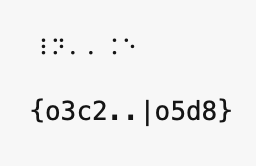
\includegraphics{../graphics/BrailleForHelloWorld.xmlWithInterpretation.png}

\caption{Braille for HelloWorld.xml with interpretation}
\label{Braille for HelloWorld.xml with interpretation}
\end{center}
\end{figure}

The interpretation shows a textual view of the contents of the previous line. {\tt o*} indicates the octave number.

% -------------------------------------------------------------------------
  \subsection{\mxml\ output}
% -------------------------------------------------------------------------

Compiling {\tt HelloWorld.msdl} to \mxml, we get:
\begin{lstlisting}[language=MusicXML]
<?xml version="1.0" encoding="UTF-8" standalone="no"?>
<!DOCTYPE score-partwise PUBLIC "-//Recordare//DTD MusicXML 3.1 Partwise//EN"
			"http://www.musicxml.org/dtds/partwise.dtd">
<score-partwise version="3.1">
    <!-- ===== Created by msdl 0.02 on Sunday 2021-05-30 @ 12:15:44 CEST from HelloWorld.msdl ===== -->
    <work>
        <work-number/>
        <work-title/>
    </work>
    <movement-number/>
    <movement-title/>
    <identification>
        <encoding>
            <software>msdl 0.02, https://github.com/jacques-menu/musicformats</software>
            <encoding-date>2021-05-30</encoding-date>
        </encoding>
        <miscellaneous>
            <miscellaneous-field name="description"/>
        </miscellaneous>
    </identification>
    <part-list>
        <score-part id="Part_One">
            <part-name/>
            <score-instrument id="Part_OneI1">
                <instrument-name/>
            </score-instrument>
        </score-part>
    </part-list>
    <part id="Part_One">
        <measure number="1">
            <attributes>
                <divisions>2</divisions>
            </attributes>
            <note>
                <pitch>
                    <step>C</step>
                    <octave>3</octave>
                </pitch>
                <duration>7</duration>
                <voice>1</voice>
                <type>half</type>
                <dot/>
                <dot/>
                <staff>1</staff>
            </note>
            <note>
                <pitch>
                    <step>D</step>
                    <octave>5</octave>
                </pitch>
                <duration>1</duration>
                <voice>1</voice>
                <type>eighth</type>
                <staff>1</staff>
            </note>
        </measure>
    </part>
</score-partwise>
\end{lstlisting}

% -------------------------------------------------------------------------
  \subsection{\guido\ output}
% -------------------------------------------------------------------------

Compiling {\tt HelloWorld.msdl} to Guido, we get:
\begin{lstlisting}[language=Guido]
{[ \staff<1> \set<autoHideTiedAccidentals="on"> \title<""> \barFormat<style= "system", range="1"> \bar<hidden="true"> \beamsOff c0/2.. \beamsOff d2/8 ]
  }
\end{lstlisting}


% -------------------------------------------------------------------------
\section{A more realistic example}
% -------------------------------------------------------------------------

Thanks to Jean Abou-Samra for providing {\tt UnPetitAir.msdl}:
\begin{lstlisting}[language=MSDL]
%{
  An explicit and implicit voices piano score
%}


% l'identification
% -----------------------------------------------

titre       "Un petit air"
compositeur "Jean Abou Samra"


% la langue pour les hauteurs de notes
% -----------------------------------------------

hauteurs francais         % par défaut: english


% la partition
% -----------------------------------------------

musique unPetitAir =
{
  |1  clef treble
      key c
      time 9/8
      r4. a,4-> <e g bf>8~ <e g bf>4.~

  |2  <e g bf>4. r2.

  %  Maintenant, je reviens en arrière pour la voix supérieure.
  |2  fs''16 gs'' fs''8 cs'' ds'' e'' b' d'' a' e'

  %  La voix inférieure s'éteint.
  |3  c''8 gs' d' c' fs' a' b' gs' b
  |4  a'8 e' a g as gs' d'( a ds)
  |5  e8( b g d' a' e'' b'' c''' b''
  |6  e'''4.) % Rien à la fin.

  %  Je décide d'ajouter une tenue de la basse.
  |5  e2.~ e4.

  %  J'ajoute encore une voix. Au passage, je change la métrique.
  |6  time 6/8
  |6  r8 e'( f') e' c'' d''

  %  Et encore un changement de métrique.
  |7  time 4/4
  |7  e''1~

  %  Je finis la phrase.
  |7  e''4 e' d''8 c'' b' a'
  |8  b'1

  %  Je retourne sur mes pas pour introduire l'ostinato.
  |7  r8 e8 f e f e c' a
  |8  r8 e8 f e c' a e f
  |9  r8 ds e ds e ds b fs

  % etc.
}
\end{lstlisting}

Jean also provided the output created by hand with \lily, see \figureRef{Un Petit Air, par Jean Abou-Samra}:
\begin{figure}[htbp]
\begin{center}
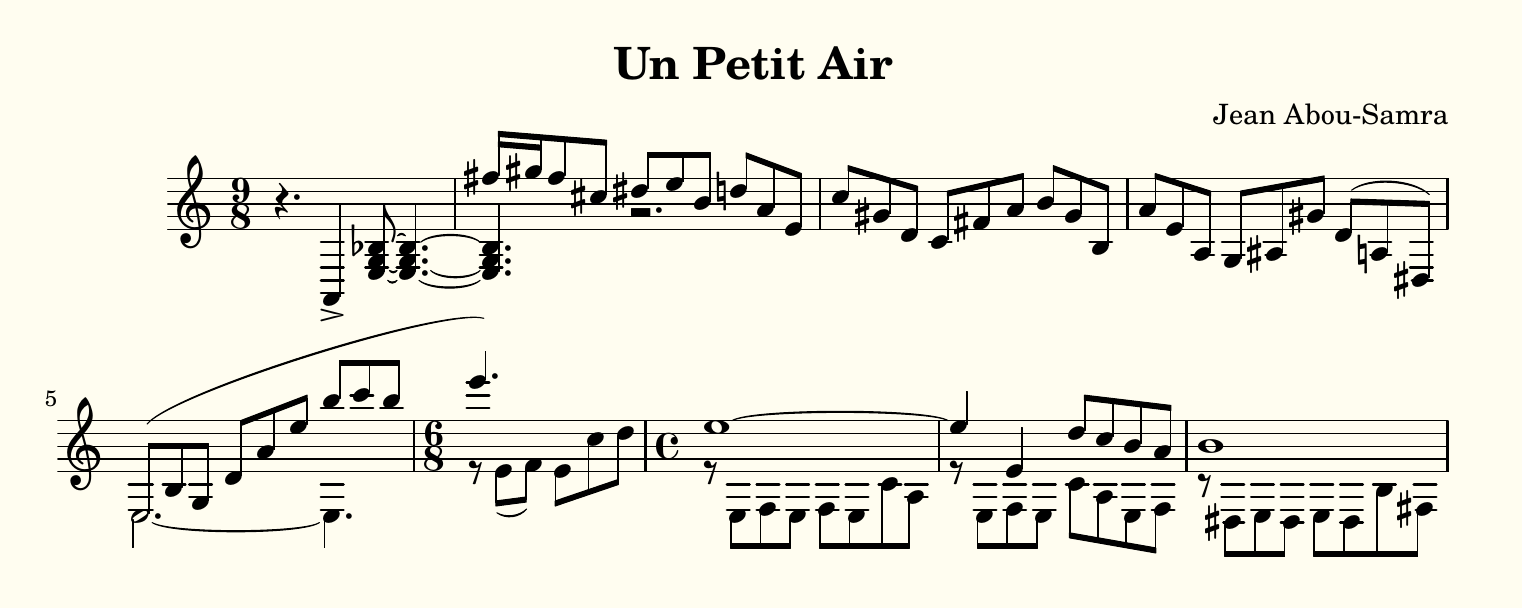
\includegraphics[scale=0.7]{../graphics/UnPetitAirParJeanAbouSamra.png}
\caption{Un Petit Air, par Jean Abou-Samra}
\label{Un Petit Air, par Jean Abou-Samra}
\end{center}
\end{figure}

% -------------------------------------------------------------------------
\section{Multi-language support}
% -------------------------------------------------------------------------


% -------------------------------------------------------------------------
  \subsection{Multi-language messages handling}
% -------------------------------------------------------------------------


% -------------------------------------------------------------------------
  \subsection{Multi-language keywords handling}
% -------------------------------------------------------------------------


% -------------------------------------------------------------------------
\section{Lexical analysis}
% -------------------------------------------------------------------------


% -------------------------------------------------------------------------
\section{Music Scores Descriptions Representation (MSDR)}
% -------------------------------------------------------------------------


% -------------------------------------------------------------------------
\section{Syntax and semantic analysis}
% -------------------------------------------------------------------------

The language-dependent keywords leads to a recursive descent parser, since {\tt flex}-generated scanners need 'fixed' keyword in the language description.


% -------------------------------------------------------------------------
  \subsection{Error recovery}
% -------------------------------------------------------------------------

The \msdLangComp\ uses a variant of the \MainIt{stopper sets} method that was present in the early Pascal and Pascal-S converters. The latter passed a set of tokens not to be overtaken to the procedures in charge of accepting the various statements in the language. Strangely enough, this was not done for declarations.

We use a stack of tokens sets that grows and shrinks in parallel with the accepting functions\index{functions}, to know more contextual informations when deciding wether to consume a token or not. The corresponding term is {it shift}
when building the analysis tables in LR technology.


